In this section we describe the results in a manner that parallels the examples in section~\ref{sec-example--dynamic-fp} with additional problem-specific details. We refer to the solutions obtained via algorithm~\ref{algo:hybrid--dynamic-fp} as the \textit{learned} solutions in the figures below. We use the Monte-Carlo method as detailed in algorithm~\ref{algo:MC--dynamic-fp} to produce reference solutions in 2 and 3 dimensions. But in the absence of analytical solutions, we refrain from calculating the difference between the reference solution and the solution produced by algorithm~\ref{algo:hybrid--dynamic-fp} since Monte-Carlo solutions can be significantly erroneous, sometimes by more than an order of magnitude compared to its counterpart, even for simple problems, as evidenced by figure~7.2 in the prequel \cite{mandal2023learning}. When dealing with high-dimensional PDEs, one widely accepted paradigm is to construct solutions that are \textit{statistically} accurate or have the correct coarse-grained structures, especially for particle-based methods in geophysics \cite{bosler2013particle}, \cite{chen2018efficient} and financial modelling \cite{cui2015particle}. We present our results in the same spirit. For each system we use a bimodal initial condition as described in section~\ref{sec-example--dynamic-fp}. Figure~\ref{fig:L63-0--dynamic-fp} shows the initial condition for the noisy Lorenz-63 system defined in \eqref{eq:p0-L63--dynamic-fp}. For ease of visualization we have integrated out the last coordinate. The symmetry of the initial condition implies the other 2D marginals are identical. The other initial conditions described in section~\ref{sec-example--dynamic-fp} are either identical or qualitatively similar. In order to produce 2D marginal densities we use Gauss-Legendre quadrature the details of which can be found in appendix~9.3 of \cite{mandal2023learning}.
\begin{figure}[!ht]
    \centering
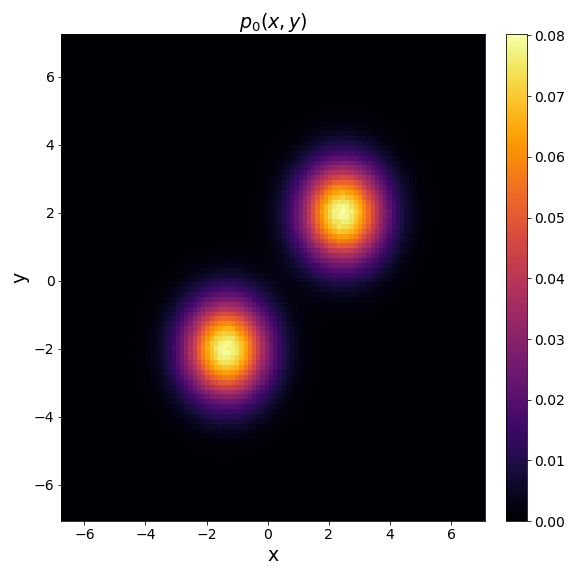
\includegraphics[scale=0.41]{dynamic-fp/plots/dynamic-plots-L63-0.png}
    \caption{Initial condition for the noisy Lorenz-63 system.}
    \label{fig:L63-0--dynamic-fp}
\end{figure}

\subsection{10D ring system} Figure~\ref{fig:10D-time--dynamic-fp} shows the computed solution for the 2$n$D ring system presented in section~\ref{ssec-2nD--dynamic-fp} for $n=5$, at time $t=0.1$. More specifically, the left panel of figure~\ref{fig:10D-time--dynamic-fp} depicts the probability density when all but the variables $x_4, x_5$ are set to $0$. For better visualization and comparison with a reference solution, the \textit{learned} solution has been normalized in a way such that,
\begin{align*}
   \int_\mathbb{R}\int_\mathbb{R} p(0.1, 0, 0, 0, 0, x_4, x_5, 0, 0, 0, 0)\, dx_4\,dx_5=1 
\end{align*}
Here we have used $M=10$, $N=10^5$ and $\mathcal D=[-2,2]^{10}$ for algorithm~\ref{algo:hybrid--dynamic-fp}.

There are no analytical solutions for this problem and classical methods are unsuitable due to the curse of dimensionality. Therefore, in order to compute a reference solution we use the careful design of the problem itself. The system described by \eqref{eq:potential-2nD--dynamic-fp} and the initial condition \eqref{eq:p0-2nD--dynamic-fp} is essentially $n$ identical, decoupled $2$D systems and we can approximately solve this $2$D system with Monte-Carlo method which is depicted in the right panel of figure~\ref{fig:10D-time--dynamic-fp}. We use $10^7$ trajectories to generate the Monte-Carlo solution. Note that, to compute the \textit{learned} solution in figure~\ref{fig:10D-time--dynamic-fp} we use a neural network approximation of $p_\infty$ obtained via the method described in \cite{mandal2023learning} rather than using the analytical version of $p_\infty$. This demonstrates the viability of algorithm~\ref{algo:hybrid--dynamic-fp} in conjunction with algorithm~6.1 of \cite{mandal2023learning} for high dimensional problems.

\begin{figure}[!ht]
    \centering
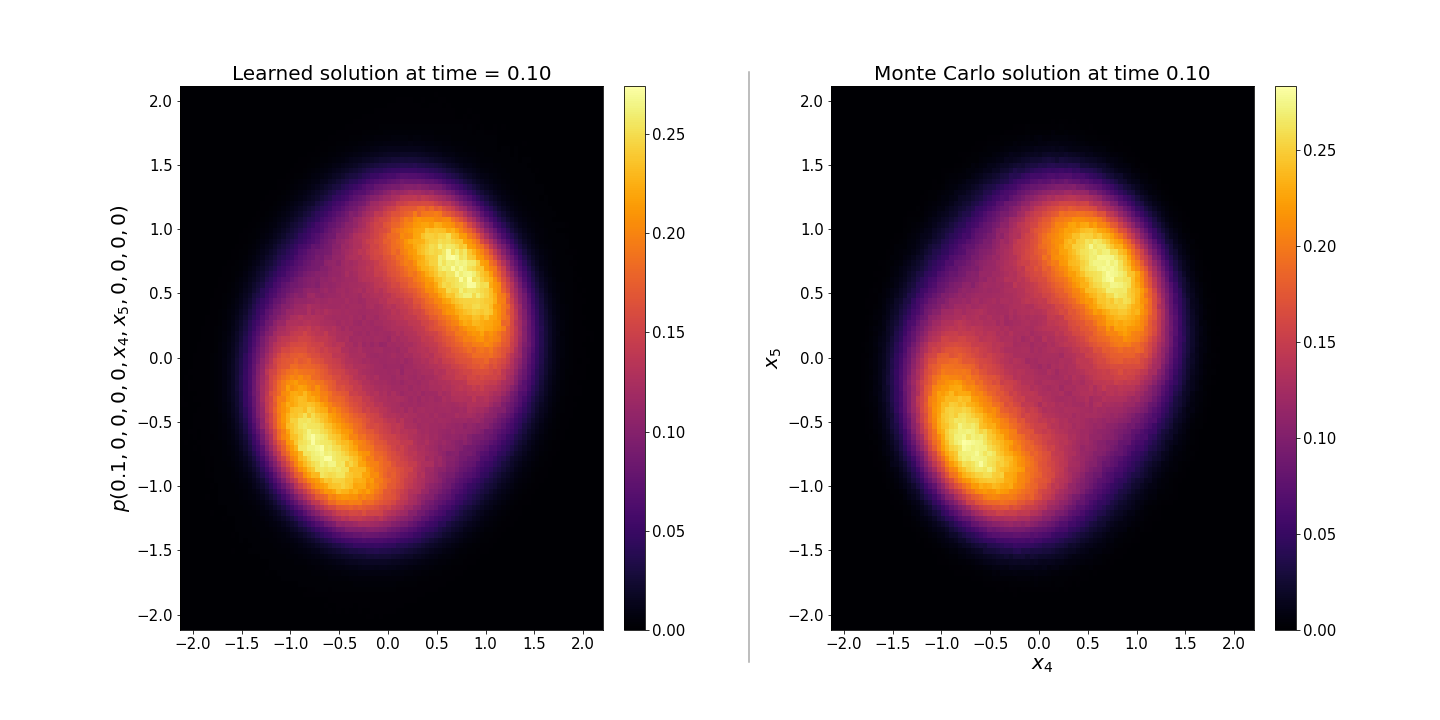
\includegraphics[scale=0.32]{dynamic-fp/plots/dynamic-plots-10D-time.png}
    \caption{Solutions for the 10D time-dependent system at time $t=0.1$. The learned solution has been normalized such that $\int_\mathbb{R}\int_\mathbb{R} p(0.1, 0, 0, 0, 0, x_4, x_5, 0, 0, 0, 0)\, dx_4\,dx_5=1$. The right panel depicts the Monte-Carlo solution for the $2$D Fokker-Planck equation corresponding to the variables $x_4,x_5$. The learned and Monte-Carlo solutions were computed using $10^5$ (pointwise) and $10^7$ trajectories respectively.}
    \label{fig:10D-time--dynamic-fp}
\end{figure}

\subsection{Noisy Lorenz-63 system}\label{ssec-res-L63--dynamic-fp}
Figure~\ref{fig:L63-time--dynamic-fp} shows the solutions for the noisy Lorenz system defined by \eqref{eq:mu-L63--dynamic-fp} at time $t=0.03$ with $\mathcal D=[-10, 10]\times[-15, 15]\times[7, 28], \Omega=[-30, 30]\times[-40, 40]\times[0, 70]$. As seen in figure~\ref{fig:xi--dynamic-fp}, $\xi(t,  \mathcal D, \Omega)\approx 1$. For easier visualization we present the 2D marginals $p(t, x, y), p(t, y, z), p(t, z, x)$. To compute $p_\infty$ in a functional form for this problem we use algorithm~6.1 in \cite{mandal2023learning}. We use $M=3$ and $N=200$ for the learned solution and $10^7$ trajectories to generate the corresponding Monte-Carlo solution. This shows that we can produce solutions with algorithm~\ref{algo:hybrid--dynamic-fp} that are comparable to Monte-Carlo method using 
several orders of magnitude fewer trajectories for each point. Both methods use $0.01$ as the step length for Euler-Maruyama.
 \begin{figure}[!ht]
    \centering
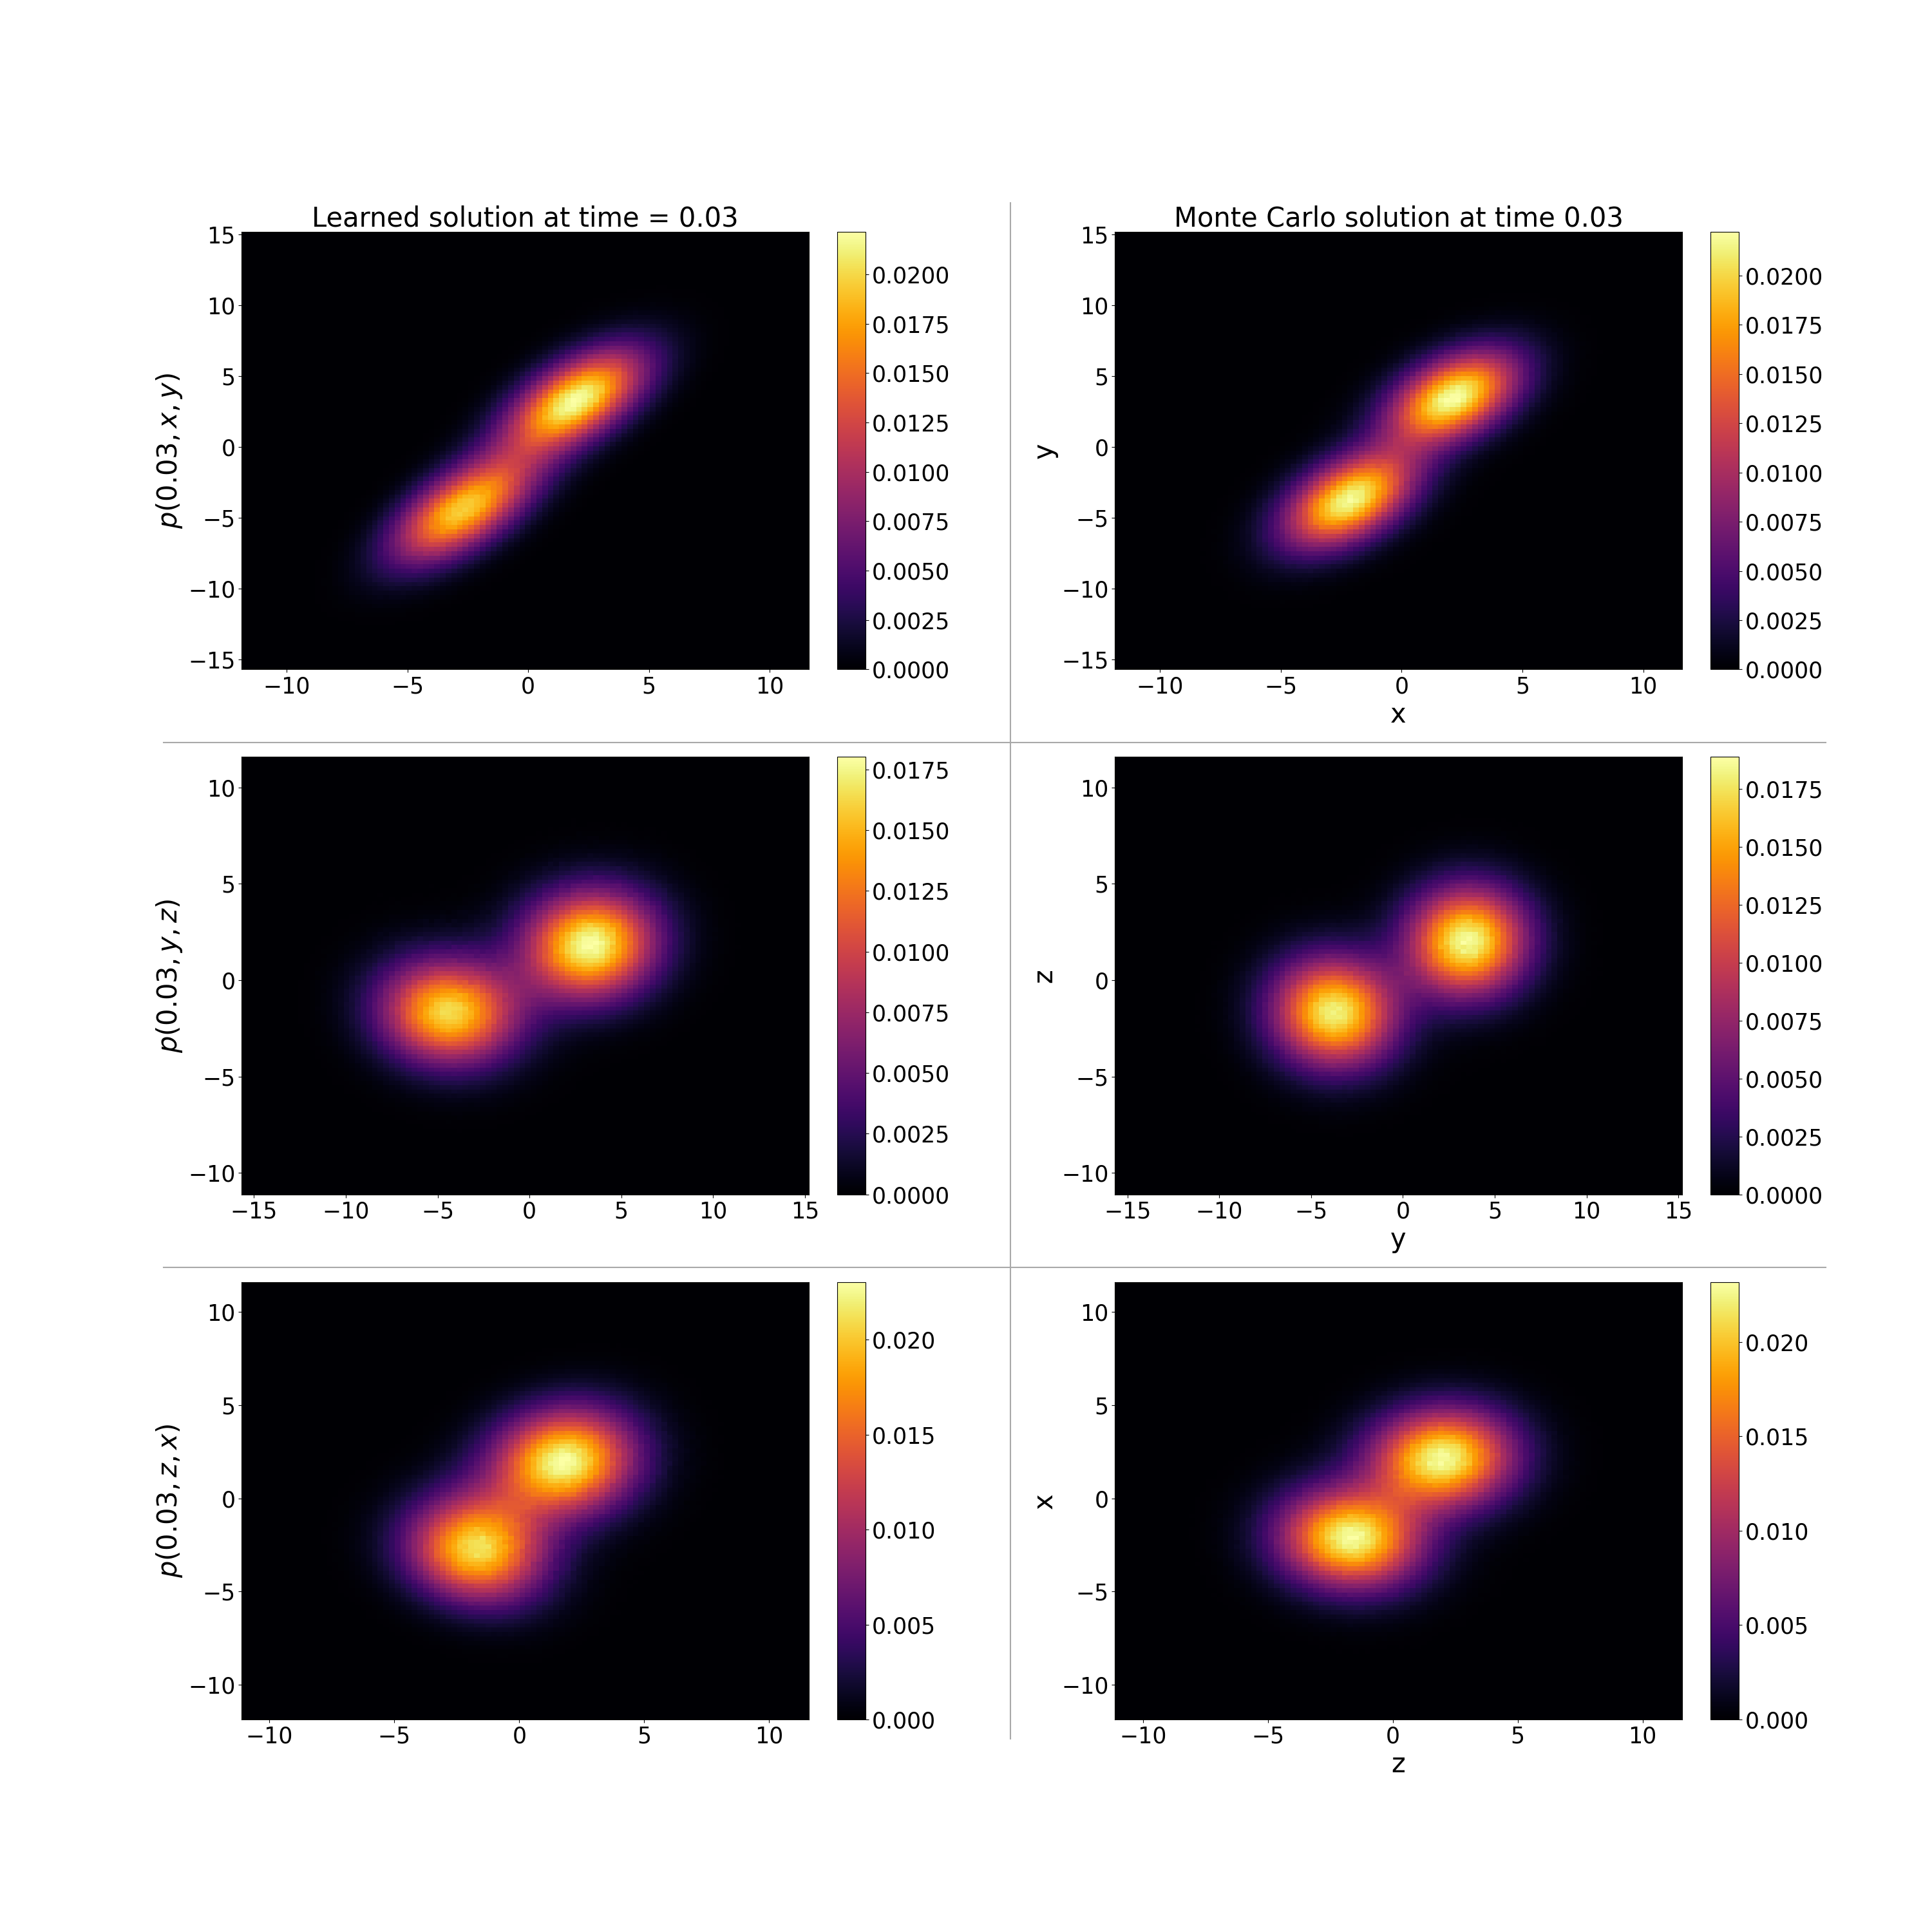
\includegraphics[scale=0.21]{dynamic-fp/plots/dynamic-plots-L63-time.png}
    \caption{Solutions for the noisy Lorenz 63 system at time t=0.03. The learned and Monte-Carlo solutions were computed using $200$ (pointwise) and $10^7$ trajectories respectively.}
    \label{fig:L63-time--dynamic-fp}
\end{figure}

\subsection{Noisy Thomas system}
Figure~\ref{fig:Thomas-time--dynamic-fp} shows the solutions for the noisy Thomas system defined by \eqref{eq:mu-Thomas--dynamic-fp} at time $t=1.0$ with $\mathcal D=[-8, 8]^3$ and $\Omega=[-10, 10]^3$. We only present $p(t, x, y)$, noting that the symmetry of the of problem renders demonstrations of the other 2D marginals redundant. We use algorithm~6.1 in \cite{mandal2023learning} for computing $p_\infty$. We use $M=10, N=50$ for the learned solution and the Monte-Carlo counterpart is computed using $10^7$ trajectories which reinstates our intuition that computing the Feynman-Kac expectation requires far fewer trajectories compared to Monte-Carlo for a similar level of accuracy.  Both methods use $0.1$ as the step length for Euler-Maruyama. In figure~\ref{fig:xi--dynamic-fp} we see that $\xi(t, \mathcal D, \Omega)\approx0.916$. So even after letting nearly $8.4\%$ of the h-SDE trajectories escape $\Omega$, we achieve a reasonable approximation.
\begin{figure}[!ht]
    \centering
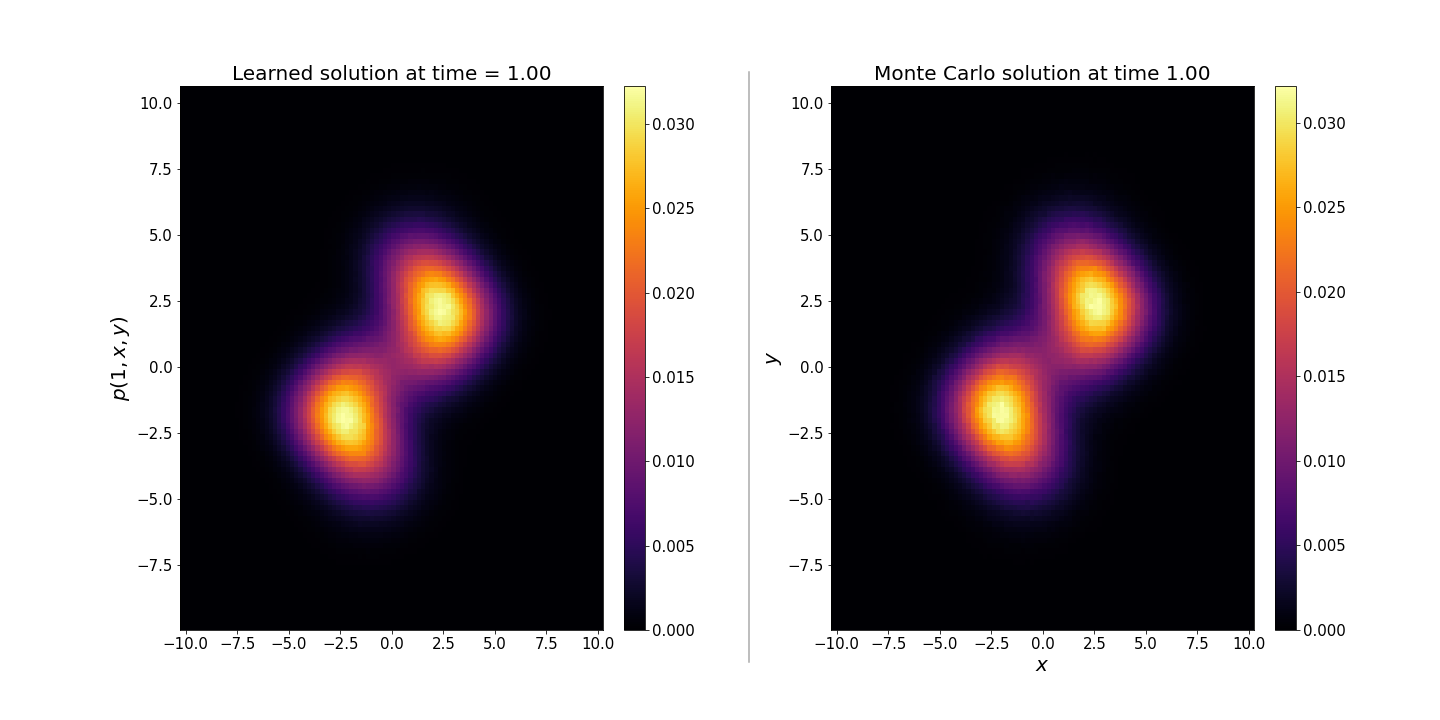
\includegraphics[scale=0.32]{dynamic-fp/plots/dynamic-plots-Thomas-time.png}
    \caption{Solutions for the noisy Thomas system at time t=1. The learned and Monte-Carlo solutions were computed using $100$ (pointwise) and $10^7$ trajectories respectively.}
    \label{fig:Thomas-time--dynamic-fp}
\end{figure}

\subsection{One step filter}
Suppose in the filtering problem described in section~\ref{ssec-1-filter-prob--dynamic-fp} we only observe $x,z$ coordinates of the noisy Lorenz 63 system and our observation noise standard deviation is $\sigma_o=5$. The one-step filtering density can be written as 
\begin{align}
    p(x_1|y_1) \propto p(x_1|x_0)p(y_1|x_1)
\end{align}
For a derivation see chapter 6 of \cite{sarkka2023bayesian} or \cite{doucet2009tutorial}. $p(x_1| x_0)$ can be thought of as the solution to the corresponding Fokker-Planck equation at time $t=g=0.03$ (the observation gap) with the initial condition being equal to the density of $x_0$,. We can calculate the likelihood $p(y_1|x_1)$ using $\sigma_o$ which lets us estimate the 2D marginals of the one-step filtering density for this problem. We calculate the solution to the Fokker-Planck equation with algorithm~\ref{algo:hybrid--dynamic-fp} and Monte-Carlo. The final one-step filtering densities are shown in figure~\ref{fig:L63-filter--dynamic-fp}. Computing the filtering density with Monte-Carlo in this way is akin to using the bootstrap particle filter, a popular nonlinear filtering algorithm, see chapter 11 of \cite{sarkka2023bayesian} or \cite{doucet2009tutorial} for more discussion on particle filters. Therefore, we refer to the Monte-Carlo estimate for the filtering density as the particle filter estimate in figure~\ref{fig:L63-filter--dynamic-fp}. We use the same $M, N$ and the same number of trajectories for Monte-Carlo as we did in section~\ref{ssec-res-L63--dynamic-fp}. It is interesting to note that the solution in figure~\ref{fig:L63-time--dynamic-fp} is bimodal whereas in the filtering density in figure~\ref{fig:L63-filter--dynamic-fp} one of the mode collapses after we make an observation.

\begin{figure}[!ht]
    \centering
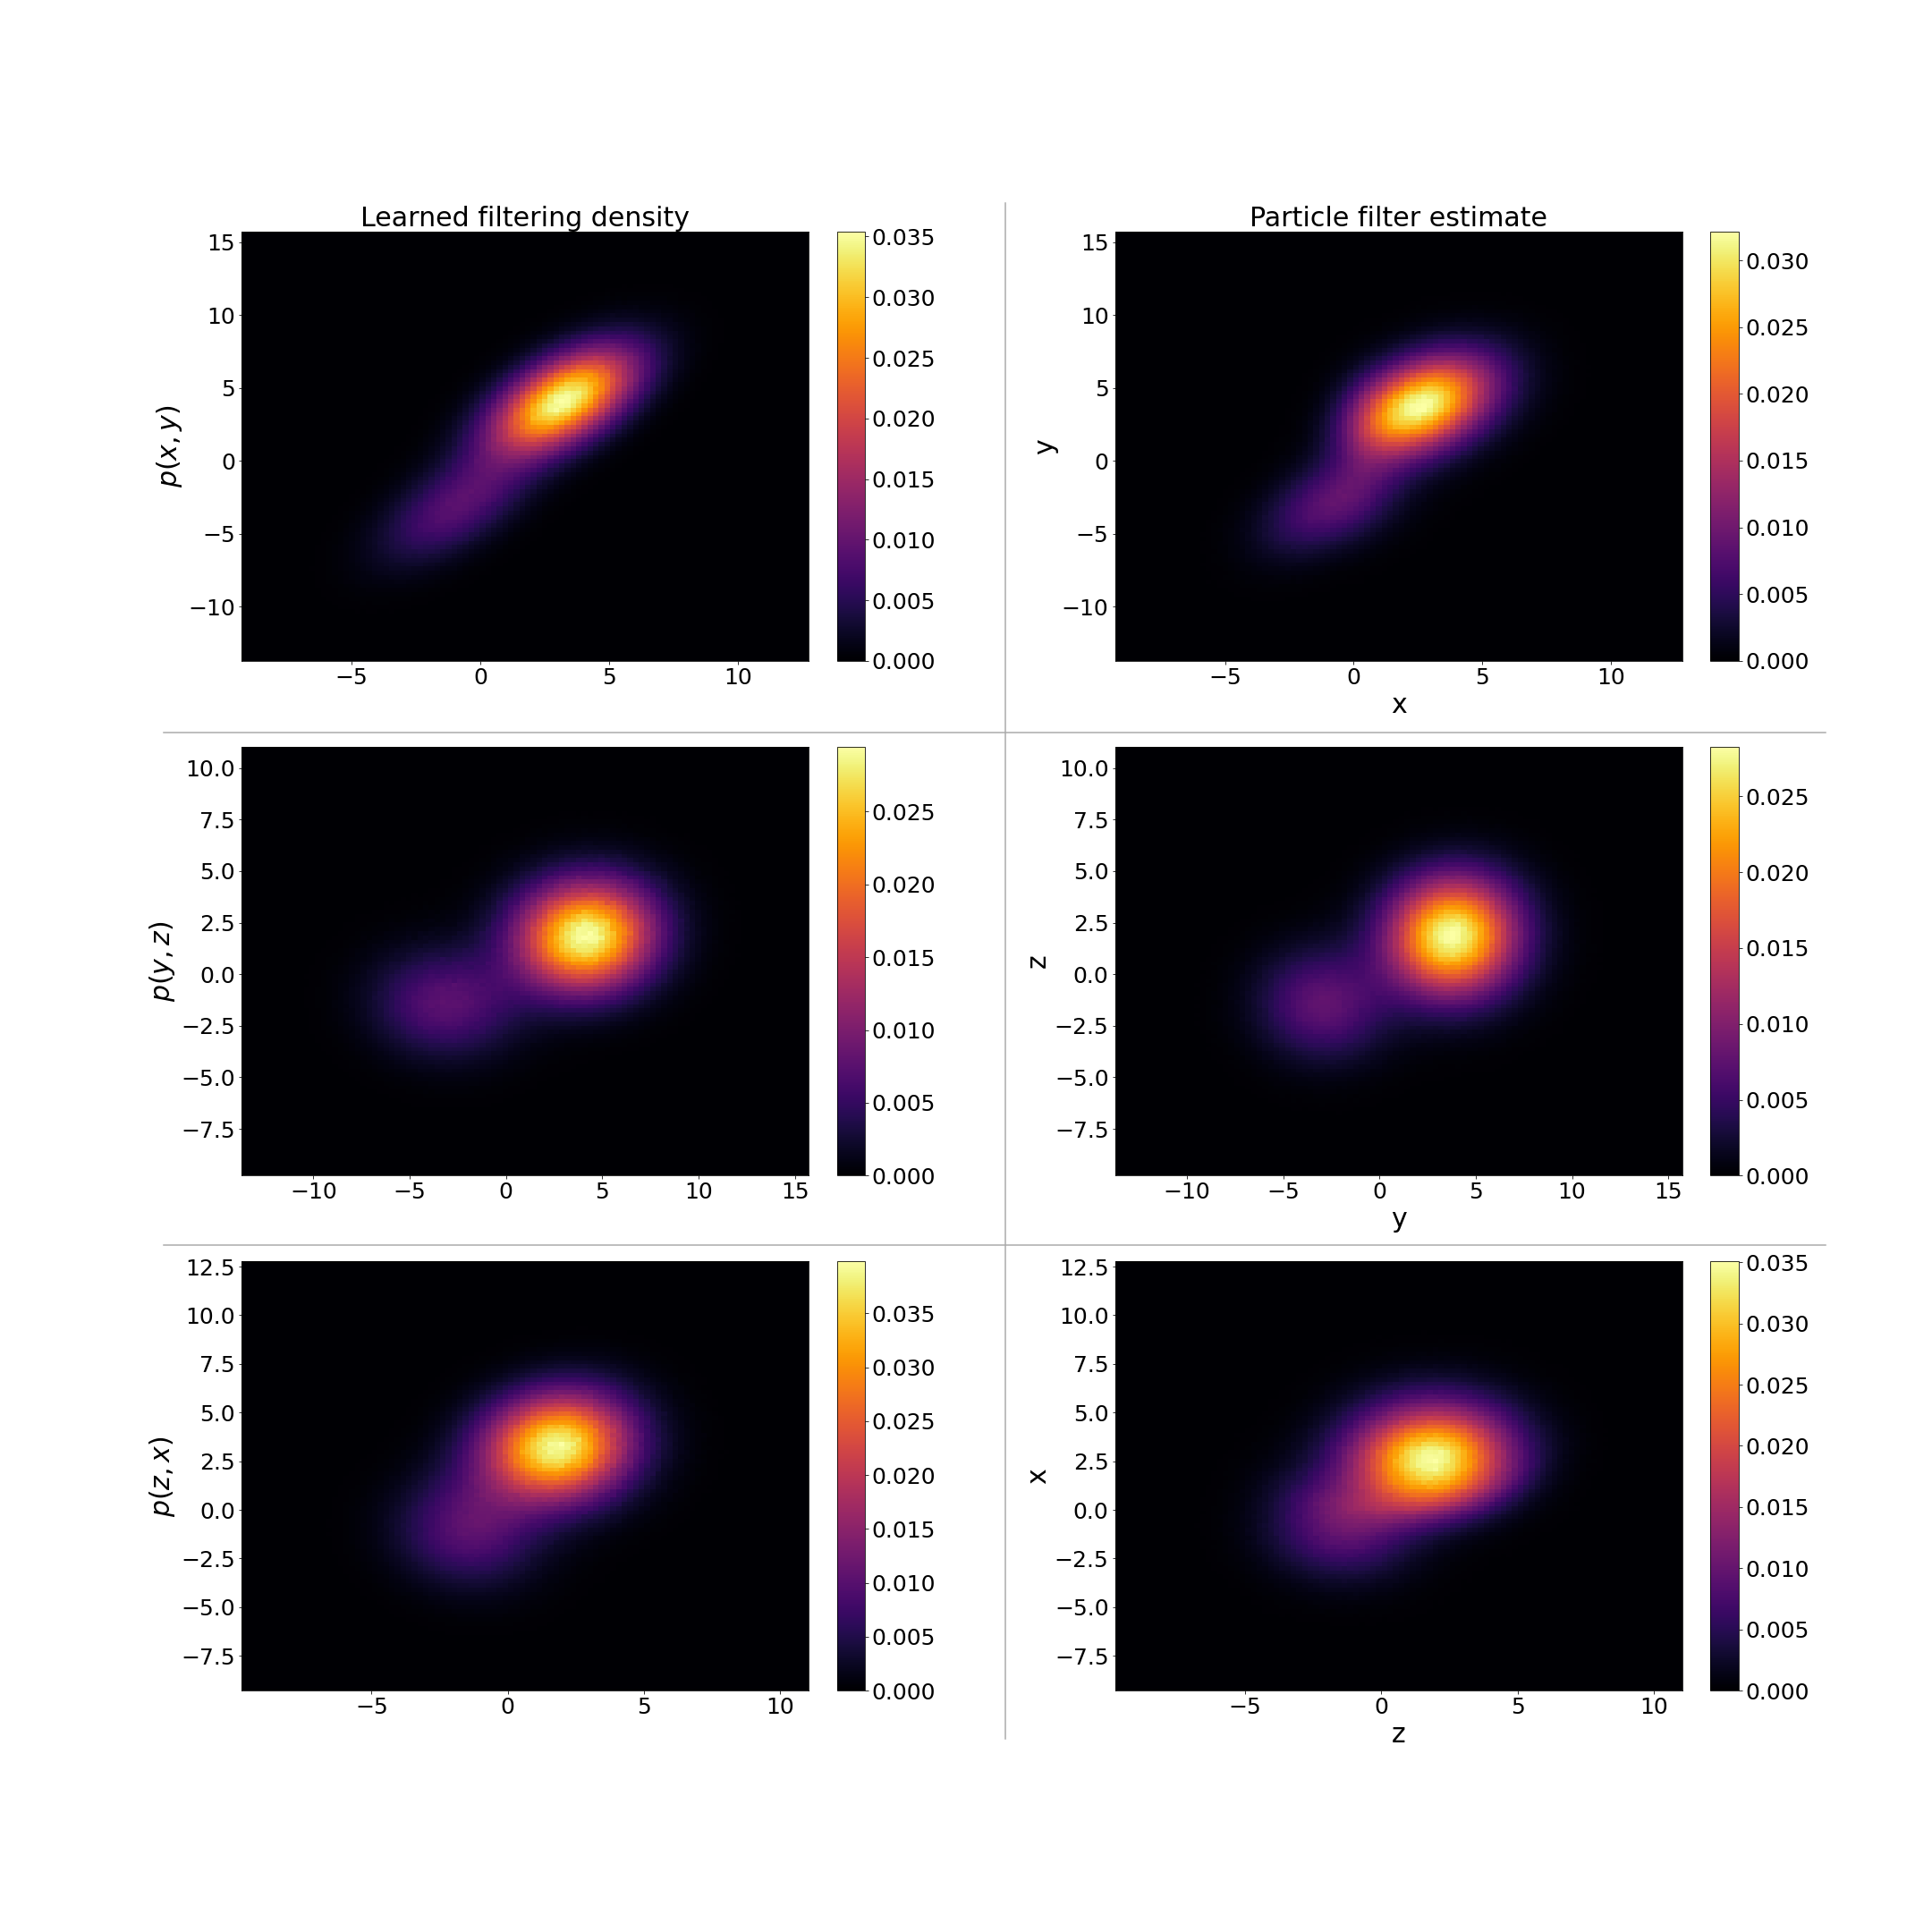
\includegraphics[scale=0.21]{dynamic-fp/plots/dynamic-plots-L63-filter.png}
    \caption{One step filtering density for the noisy Lorenz 63 system. The learned and particle filter solutions were computed using $200$ (pointwise) and $10^7$ trajectories respectively.}
    \label{fig:L63-filter--dynamic-fp}
\end{figure}